\documentclass[a4paper]{scrreprt}

\usepackage{scrhack}
\usepackage{graphicx}
\usepackage[utf8]{inputenc}

\addtokomafont{titlehead}{\flushright}
\addtokomafont{subject}{\vspace{3cm}\flushleft}
\addtokomafont{title}{\flushleft}
\addtokomafont{subtitle}{\flushleft}
\addtokomafont{author}{\flushleft\setlength{\tabcolsep}{0pt}}
\addtokomafont{date}{\flushleft}
\addtokomafont{publishers}{\flushleft}

\titlehead{
\includegraphics[scale=2]{logo_en}}
\subject{Software Engineering and Design}
\title{Design Thinking}
\subtitle{Mental Health Care Patient Management System (MHC-PMS)}
\author{
\begin{tabular}{l}
\normalfont\bfseries{Team White:}\\
Dellsperger Jan\\
Ellenberger Roger\\
Sheppard David\\
Sidler Matthias\\
Spring Mathias\\
Thöni Stefan
\end{tabular}
}
\date{\today}
\publishers{Version 1.0}

\begin{document}

\begin{titlepage}
	\maketitle
\end{titlepage}






\tableofcontents

\bigskip

\section*{Über dieses Dokument}
Dieses Dokument beschreibt den Design Thinking Prozess von \textit{Team White}. Das Dokument hält das Vorgehen der einzelnen Schritte über mehrere Iterationen hinweg fest. Die Ergebnisse sind im Kapitel \textit{Ergebnisse} dokumentiert. Die Details der Interviews sind nicht in diesem Dokument zu finden.

\chapter{Prozess-Ablauf}
\section{Iteration 1}
Wir haben uns bei der ersten Iteration darauf konzentriert, überhaupt den Prozess Design Thinking kennenzulernen. Ganz nach dem Tipp des Dozenten haben wir einfach begonnen den Prozess zu leben. Beim Designen der ersten Storyboards bemerkten wir, dass noch zu wenig klar ist, was die Zielgruppe Manager ausser einem guten Reporting sonst noch alles braucht.

\subsection*{16.03.2016}
\paragraph{Research}
Vor dem eigentlichen Scoping hat jedes Teammitglied unabhängig 15 Minuten recherchiert. So fanden wir heraus, welche Fragen offen sind, welche Zielpersonen die Software zukünftig brauchen könnten und evtl. auch bereits erste Probleme die zu lösen sind.


\paragraph{Scoping}
Auf Basis der ersten Erkenntnisse führten wir das erste Scoping durch.


\paragraph{Research}
In einer zweiten Analyse recherchierten alle Teammitglieder nach Domänen-Wissen zu psychiatrischer Betreuung, Konkurrenzprodukten und möglichen Nutzern.


\paragraph{Scoping}
Scoping erweitert. Die Haupt-Frage ist, ob unsere Benutzergruppe noch mehr Anforderungen hat als ein gutes Reporting. Hierzu wollen wir in weiteren Recherchephasen mehr herausfinden. Zudem suchten wir schon etwas spezifischer, welche Reports und Statistiken ein Benutzer der Software brauchen könnte.


\paragraph{Syntesis}
Erste Personas erstellt. Mehrere davon auf Anhieb verworfen.


\paragraph{Design}
Jederes Teammitglied hatte 15 Minuten Zeit, um Storybaords zu erstellen. Die Ergebnisse wurden diskutiert. Wir wissen immer noch zu wenig genau, was der User braucht.


\section{Iteration 2}
Auch in der zweiten Iteration wollten wir die Hauptfrage der Iteration 1 klären: Was ausser guten Reports brauchten die Nutzer noch? Die individuelle Recherche Zuhause hat nicht die gewünschten Ergebnisse geliefert. Daher fuhren wir fort, einfach den Prozess zu durchlaufen und Ideen zu suchen, indem wir uns mit dem Thema beschäftigten. Wir machten nochmals Storyboards und kurz darauf erste Prototypen. Wir sahen das erste Mal, was sich welches Teammitglied als Lösung vorstellte.

\subsection*{16.03.2016}
\paragraph{Research}
Jedes Teammitglied betreibt individuelle Research als "Hausaufgabe" (je nach verfügbarer Zeit).


\subsection*{18.03.2016}
\paragraph{Design}
Weitere Storyboards entwickelt.


\paragraph{Prototype}
Individuell 30 Minuten Prototypen entwickelt und anschliessend verglichen. Grosse Unterschiede zwischen den einzelnen Prototypen, da jedes Teammitglied andere Vorstellungen des Endprodukts hat.

\paragraph{Research}
Aus der Diskussion der Prototypen ging hervor, was jedes Teammitglied für eine Lösung vor Augen hatte. Dies basierte meistens auf einer bereits eingesetzten Lösung aus dem Privat- oder Geschäftsumfeld. 

\paragraph{Syntesis}
Erkenntnisse aus Prototypen in Anforderungsanalyse zusammengetragen.



\section{Iteration 3}
In dieser Iteration hatten wir ein weiteres Instrument für die Research-Phase zu Verfügung: Interviews. Wir konnten diese auch nutzten, um weitere Anforderungen der Benutzer abzuholen. Es hat sich dabei hauptsächlich bestätigt, dass gute Reports das wichtigste sind. Nebenbei wird oft gewünscht, direkt eine Akte eines Patienten zu analysieren oder einfach zu exportieren, um einer Krankenkasse zuzustellen.
In dieser Iteration entstanden wirklich brauchbare Prototypen, welche wir auch mittels Testpersonen validieren konnten.

\subsection*{18.03.2016}

\paragraph{Research}
Interviewfragen im Plenum vorbereitet.

\subsection*{22.03.2016}
\paragraph{Research}
Interviews vorbereitet und Fragenkatalog überarbeitet. Weiteres vorgehen abgesprochen. Wichtig für das weitere Vorgehen ist es, Informationen zu erhalten aus denen wir konkrete Benutzeranforderungen erstellen können.


\subsection*{23.03.2016}
\paragraph{Research}
Interview mit Mitarbeiten aus dem Managements eines Spitals und einer Klinik.


\subsection*{24.03.2016}
\paragraph{Research}
Interview mit einer Abteilungsleiterin einer Pflegestätte. Anschliessendes Auswerten der Informationen.

\subsection*{25.03.2016}
\paragraph{Syntesis}
Team die Ergebnisse aus den Interviews mitgeteilt. Mit diesen Erkenntnisse zwei Personas definiert und ein Mindmap mit User-Requirements erstellt. Resultat in diesem Bericht dokumentiert.

\paragraph{Design}
Jedes Teammitglied hat zwei oder mehr Storyboards erstellt. Diese im Plenum besprochen und die besten ausgewählt. 

\paragraph{Prototype}
Zu den drei besten Storyboards Prototypen erstellt. Arbeit in Zweiergruppen (dellj1/shepd1, eller1/sprim5, sidlm3/thons1).


\subsection*{26.03.2016 - 30.03.2016}
\paragraph{Validation}
Prototypen mit Testpersonen validiert. Zu den Tests jeweils ein Testprotokoll geführt.


\paragraph{Prototype}
Prototypen, wo nötig, ausgebessert und erweitert.


\paragraph{Validation}
Erneute Tests mit verbesserten Prototypen durchgeführt.



\chapter{Ergebnisse}
\section{Scoping}

\subsection{Projekt Scope}
Die Hauptzielgruppe für die Software ist vorgegeben: Manager.

\bigskip


\textbf{Fragestellungen die Untersucht werden sollen:}
\begin{itemize}
\item Welche Personen gehören zu unserer Zielgruppe? (Charakter, sozialer Status, Alter, Geschlecht, Ausbildungsniveau, etc.)
\item Inwiefern unterscheiden sich die Leute in unserer Zielgruppe? Haben einige Personen deutlich abweichende Anforderungen als andere?
\item Was sind die Hauptfragen des Managements, welche die Software helfen soll zu beantworten?
\item Welche Institutionen werden die Software verwenden? (Spitäler, Krankenkassen, Bundesämter...)
\item Welche rechtlichen Grundlagen muss die Lösung erfüllen?
\end{itemize}


\textbf{Fragen zum Alltag des Benutzers:}

\begin{itemize}
\item Welche Einblicke / Ergebnisse (aus den gesammelten Daten) braucht der Benutzer?
\item Welche Probleme hat der Benutzer?
\item Welchen Hintergrund hat der Benutzer? (Karriere, Leistungsausweis, Informatikkenntnisse)
\item Gibt es Benutzer die oft repetitive Tätigkeiten ausführen?
\item In welche Position arbeitet der Benutzer?
\end{itemize}

\subsection{Nicht im Projekt Scope}

\begin{itemize}
\item Anforderungen die explizit nicht mit \textit{Mental Health} zusammenhängt
\item Bedürfnisse von Benutzern aus der Administration (Rechnungsstellung, Patientenverwaltung, etc.)
\item Aus der Aufgabenstellung selber folgt, dass es keine Datenerfassung geben wird im Bereich Management.
\item Es werden keine Funktionalitäten zum unterstützen von Ärtzten evaluiert. 
\end{itemize} 

\subsection{Erfolgsfaktoren}

\begin{itemize}
\item Anforderungen und Probleme der Benutzer verstehen
\item Fokus auf Project-Scope legen (keine Anforderungen umsetzen, die nicht für unsere Zielgruppe bestimmt sind)
\item Einhalten der Vorgaben (u.a. Timeline)
\end{itemize} 


TODO: Erfolgsfaktoren, Restriktionen(timeline etc.)

\section{Research}
\paragraph{Recherche-Vorgehen:} 
\begin{itemize}
\item Internet-Recherche
\item Interviews
\end{itemize}


\paragraph{Recherchethemen:} 
\begin{itemize}
\item Benutzer-Rollen
\item Grundlegende Probleme in Healt-IT (Stichwörter: ACM CHI, Health IT (HIT), Useability in HIT)
\item Lösungen von Konkurrenten
\item Rechtliche Grundlagen
\end{itemize}

\subsection{Benutzer-Rollen}
Die Anforderungen der Benutzer sind sehr unterschiedlich, je nach grösse der Klink. Daher ist die Benutzergruppe Manager, eher als Rolle zu verstehen, die von verschiedenen Benutzern ausgeübt werden. Die Applikation wird daher nicht immer gleich benutzt (bspw. sind für eine kleine Praxis andere Informationen von Bedeutung als für ein Spital).\footnote{Informationen aus Interview vom 23.03.2016}

\paragraph{Anforderungen der Benutzer}
\begin{itemize}
\item Rollenkonzept für Benutzer
\item Planungsfunktionalitäten
\item Auswertungen / Reports zu Finanzen und Pflege
\item Reports auf Ebene der Patienten (Export von Patientenakten)
\item Prognosen und Vorhersagen (automatisiert)
\end{itemize}


\subsection{Probleme in Health-IT}
\paragraph{Patientensicherheit} In Health IT ist eines der grössten Probleme die Patientensicherheit. Viele Anbieter sind besorgt, dass ein Softwarefehler Leben kosten kann. Zudem ist es schwer eine Balance zwischen Benutzerfreundlicher Bedienung und Sicherheit zu finden.\footnote{http://interactions.acm.org/archive/view/july-august-2012/measuring-usability-in-healthcare-it}
Für unsere Zielgruppe ist dieser Punkt aber weniger von Bedeutung.

\paragraph{Heterogene IT Systeme} Health IT ist ein sehr komplexes Themengebiet, da die zusammenarbeitenden Systeme sehr heterogen sind. \footnote{Informationen aus Interview vom 23.03.2016}



\subsection{Konkurrenzprodukte}
\paragraph{Insights} Eine Anforderung an die Software ist, durch gutes Reporting Einblicke zu erhalten, die vorher nicht so einfach oder gar nicht möglich waren. Das Oberthema dazu ist \textit{Analytics} und \textit{Business Intelligence}. Ein bekanntes Produkt in diesem Bereich ist Microsoft PowerBI\footnote{https://powerbi.microsoft.com/en-us/} .

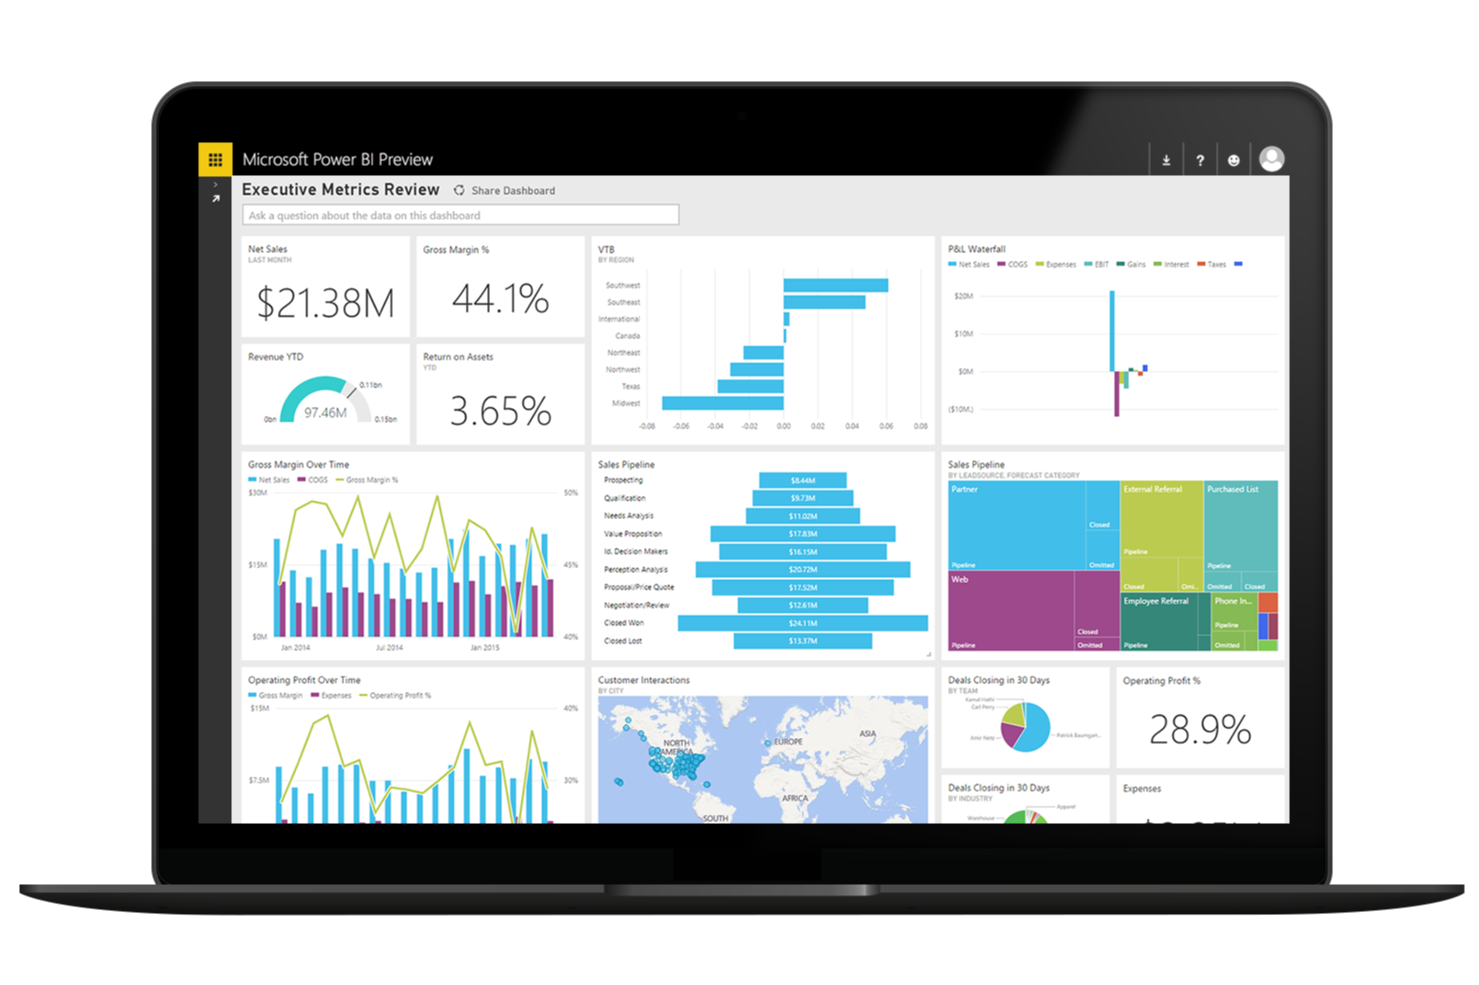
\includegraphics[width=0.6\textwidth]{img/research_ms-powerbi.png}

Microsoft bietet hier ein Werkzeug, mit dem sich bereits gesammelte Daten effektiv analysieren und visualisieren lassen. Die generierten Berichte lassen sich über einen Webbrowser oder ein Mobiles Endgerät einsehen. Der Dienst läuft in der Cloud ist daher nicht geeignet für das direkte Verarbeiten von Patientendaten.

\bigskip

Das Schweizer Unternehmen \textit{Erne Consulting} bietet für ihre eHealth-Lösung \textit{Polypoint} für diesen Zweck eine Reporting-Erweiterung an \footnote{http://polypoint.ch/}.

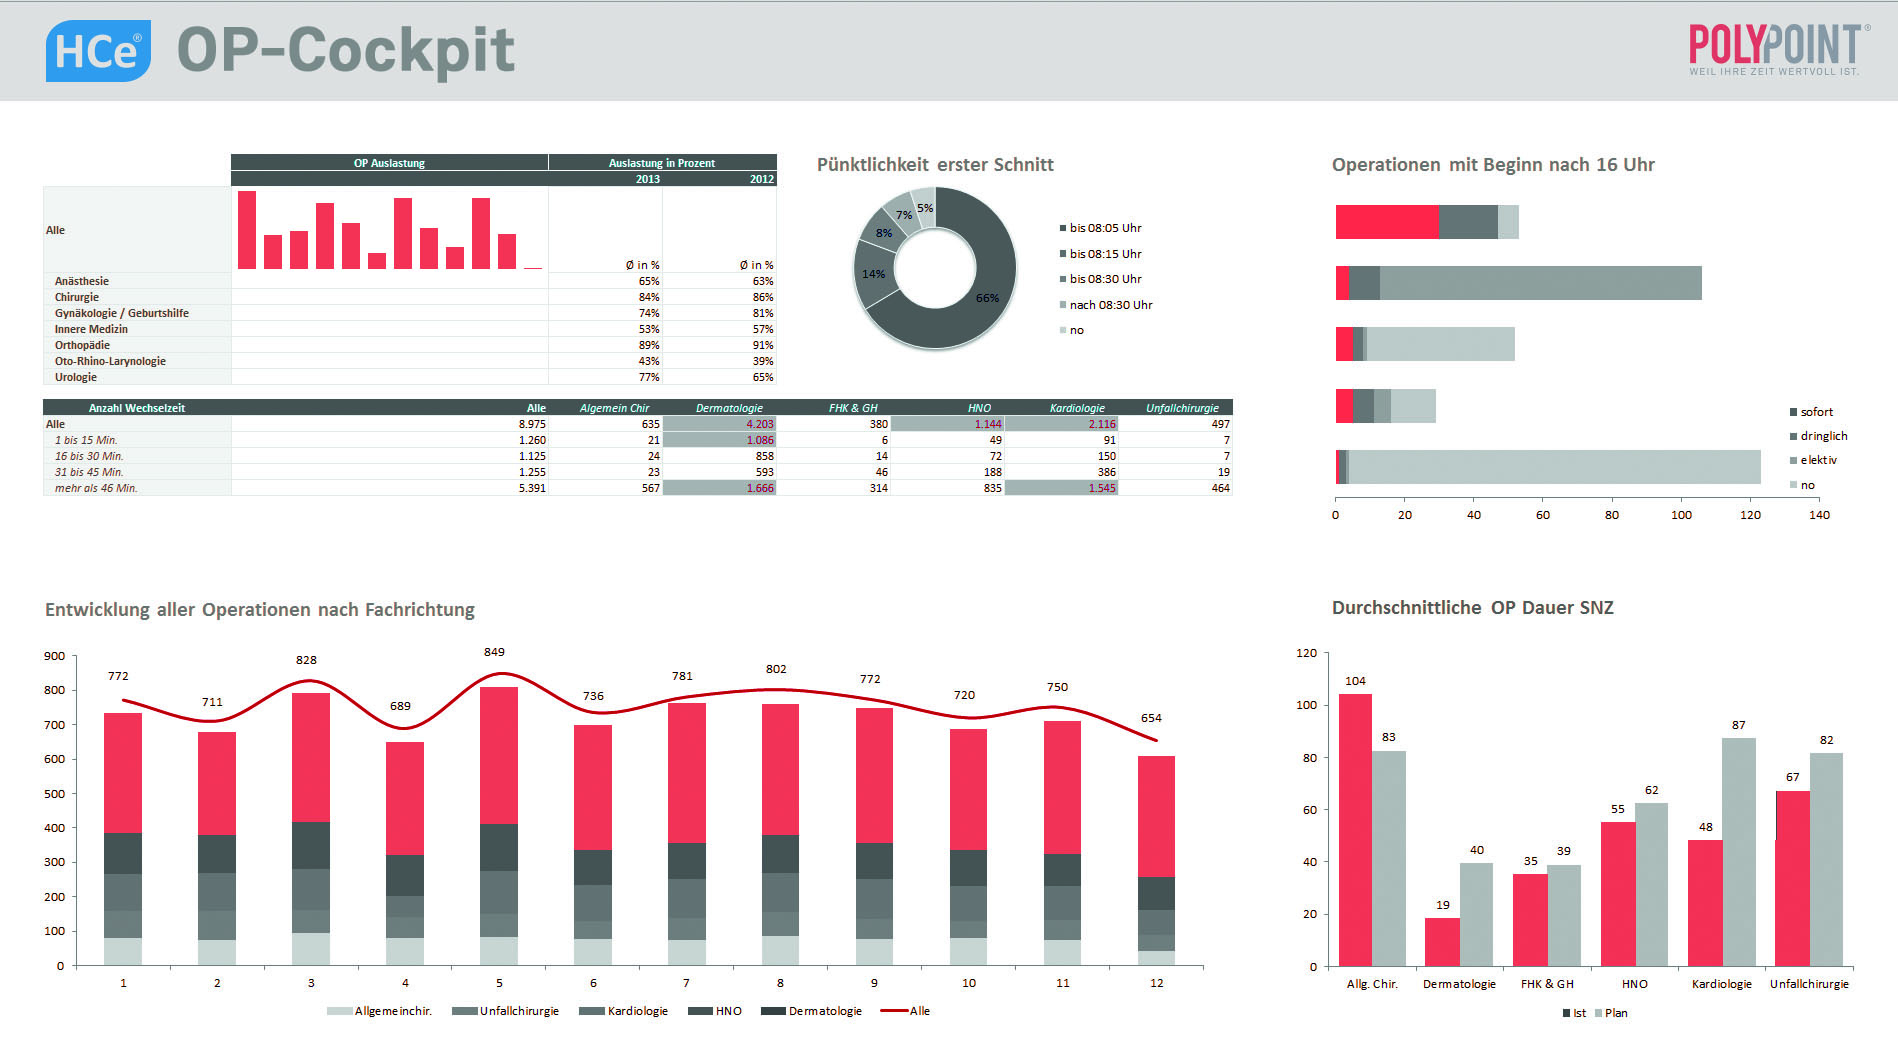
\includegraphics[width=0.75\textwidth]{img/research_polypoint_op-cockpit.jpg}



\subsection{Rechtliche Grundlagen}
Informationen zu den rechtlichen Anforderungen erhielten wir im Interview vom 23. März. Aktuell ist dies keine Benutzeranforderung sondern ein Domain-Requirement.



\section{Syntesis}
Gerade in den Interviews wurde ersichtlich, dass die Zielgruppe Manager mehr eine Rolle ist, als eine konkrete Person. Je nach Grösse der Betreuungseinrichtung gibt es keinen expliziten Manager. In kleineren Einrichtungen hat auch ein Arzt die Rolle Manager inne.
Die Anforderungen gehen je nach Grösse des Zielkunden auseinander.

\subsection{Personas}
Aus den gewonnen Erkenntnissen der Recherche-Phase haben wir uns auf zwei Personas festgelegt:

\paragraph{Ariane} leitet die Abteilung Pflege in einer grossen Betreuungseinrichtung für Personen mit psychischen Störungen. Damit übernimmt sie die Personalplanung und ist verantwortlich, dass die Prozesse in der Einrichtung funktionieren. Aufgrund ihrer grossen Führungsspanne arbeitet sie sehr strukturiert und sucht stets Möglichkeiten Zeit zu sparen.

Sie will zudem stets informiert sein über aktuelle Notfälle oder sonderbare Ereignisse im Zusammenhang mit den Patienten. Sie will stets die Hintergründe kennen, warum etwas passiert und überlässt nichts dem Zufall.


\paragraph{Bruno} ist leitender Arzt einer kleinen Betreuungseinrichtung für ambulante Behandlung von Personen mit psychischen Störungen. Er leitet die Praxis alleine. Unterstützend für die Behandlung, den Empfang und die Büroarbeit arbeiten zwei Assistentinnen unter seiner Führung. Er ist sehr interessiert an Finanzzahlen, um nicht aus Sicht der Krankenkassen einen zu hohen Umsatz zu generieren. Der Umgang untereinander ist sehr familiär und basiert auf erwähnenswert viel Vertrauen.


\subsection{Main Features (User Requirements)}
Aus den Ergebnissen der letzten Phase (Interviews, Recherche) und Diskussionen im Team\footnote{Mindmap des Brainstormings abgelegt unter /doc/task03/img/mindmap-mainfeatures.jpg} ergaben sich folgende User Requirements:

\paragraph{Dashboard}
Es soll ein Dashboard geben, in dem die wichtigsten Kennzahlen graphisch dargestellt sind. Dieses Dashboard soll vom Benutzer selber auf seine Bedürfnisse angepasst werden. 

Zusätzlich dazu soll es die Möglichkeit geben, ab einer bestimmten Limite eine Alarmierung auszulösen. 

\paragraph{Statistische Auswertung}
Bestimmte Statistiken sollen aus den vorhandenen Daten generiert und angezeigt werden können (Beispiele: Periodenvergleich, Überzeit der Mitarbeiter). Der Benutzer muss in der Lage sein, sich diese automatisiert in regelmässigen Abständen per Email zukommen zu lassen.

\paragraph{Daten Export/Import}
Da verschiedene Organisationen (Krankenkassen, Bundesamt für Statistik, etc) an gewissen Daten interessiert sind, müssen diese in einem für sie interpretierbaren Format exportiert werden können. 

\paragraph{Pesonal Verwaltung}
Eine Haupttätikeiten der Manager ist das Verwalten und Monitoren der Angestellten. Um dies zu unterstützen, sollte überprüft werden können, was die Angestellten in einer Zeitspanne bearbeitet haben. 

Um die Planung zu unterstützen, sollen die geplanten Tätigkeiten der Angestellten dargestellt werden können. (Z.B. in einem Gantt-Diagramm)

\paragraph{Pflege und Therapie}
Die Wirksamkeit von den verschiedenen Medikamenten und Therapien kann mit Hilfe der statistischen Auswertungen aufgezeigt werden können. Die Häufigkeit von verschiedenen Vorkommnissen (Eintritte, Austritte, Notfälle) soll dargestellt werden. 

\paragraph{Finanzverwaltung}
Um die Verwaltung der Finanzen zu unterstützen soll eine Auswertung über die Einnahmen sowie Ausgaben erstellt werden können. Ausserdem sollen diese über verschiedene Perioden verglichen werden können.

\pagebreak

\section{Design}
Über die verschiedenen Iterationen im Design-Thinking Prozess haben wir diverse Storyboards \footnote{Alle Storyboards sind  abgelegt unter /doc/task03/storyboards\_personas\_prototypes, geordnet nach Iterationen} erstellt. Dabei gab es von skurrilen bis sehr realitätsnahen Storyboards fast alles. In diesem Dokument sind lediglich die drei Storyboards eingebunden, welche auch für die weiterführenden Prototypen verwendet wurden. Welche Prototypen das sind, haben wir im Plenum abgestimmt.

\paragraph{Storyboard 1 und 2} beide mit Fokus aus Reporting



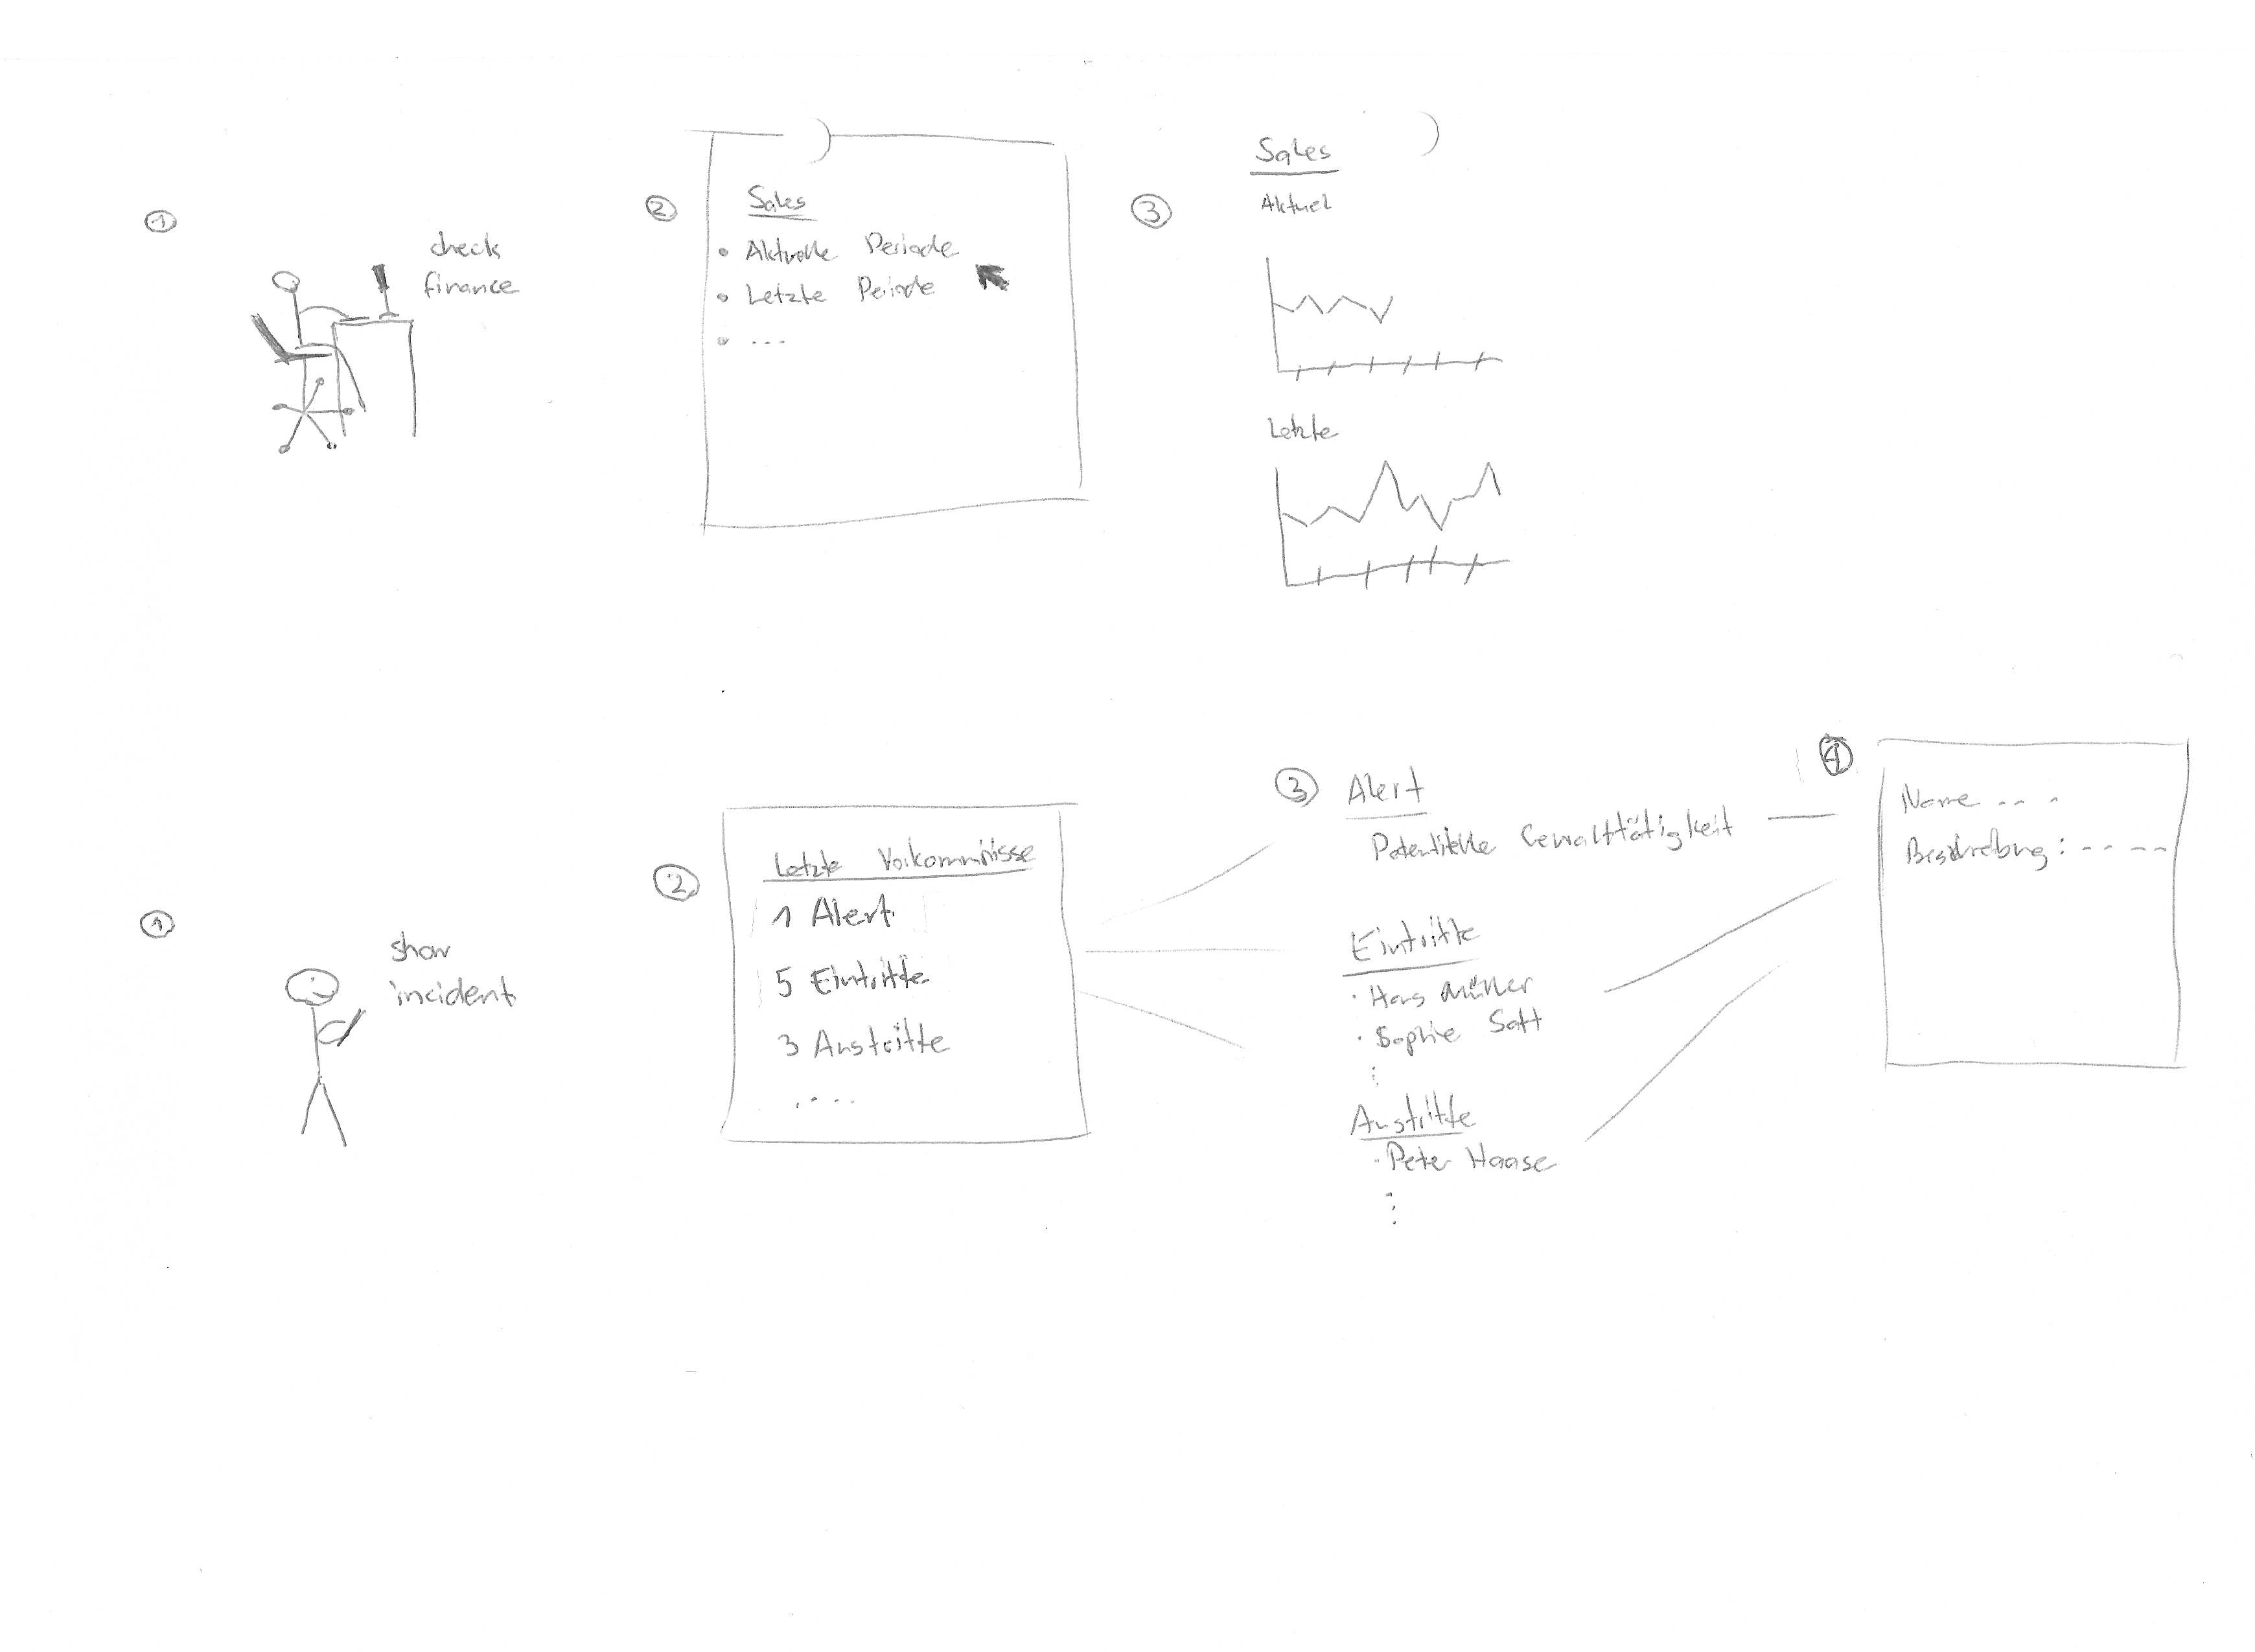
\includegraphics[width=1\textwidth]{storyboards_personas_prototypes/iteration3/sidlm3_storyboard2+3.png}

\paragraph{Storyboard 3}

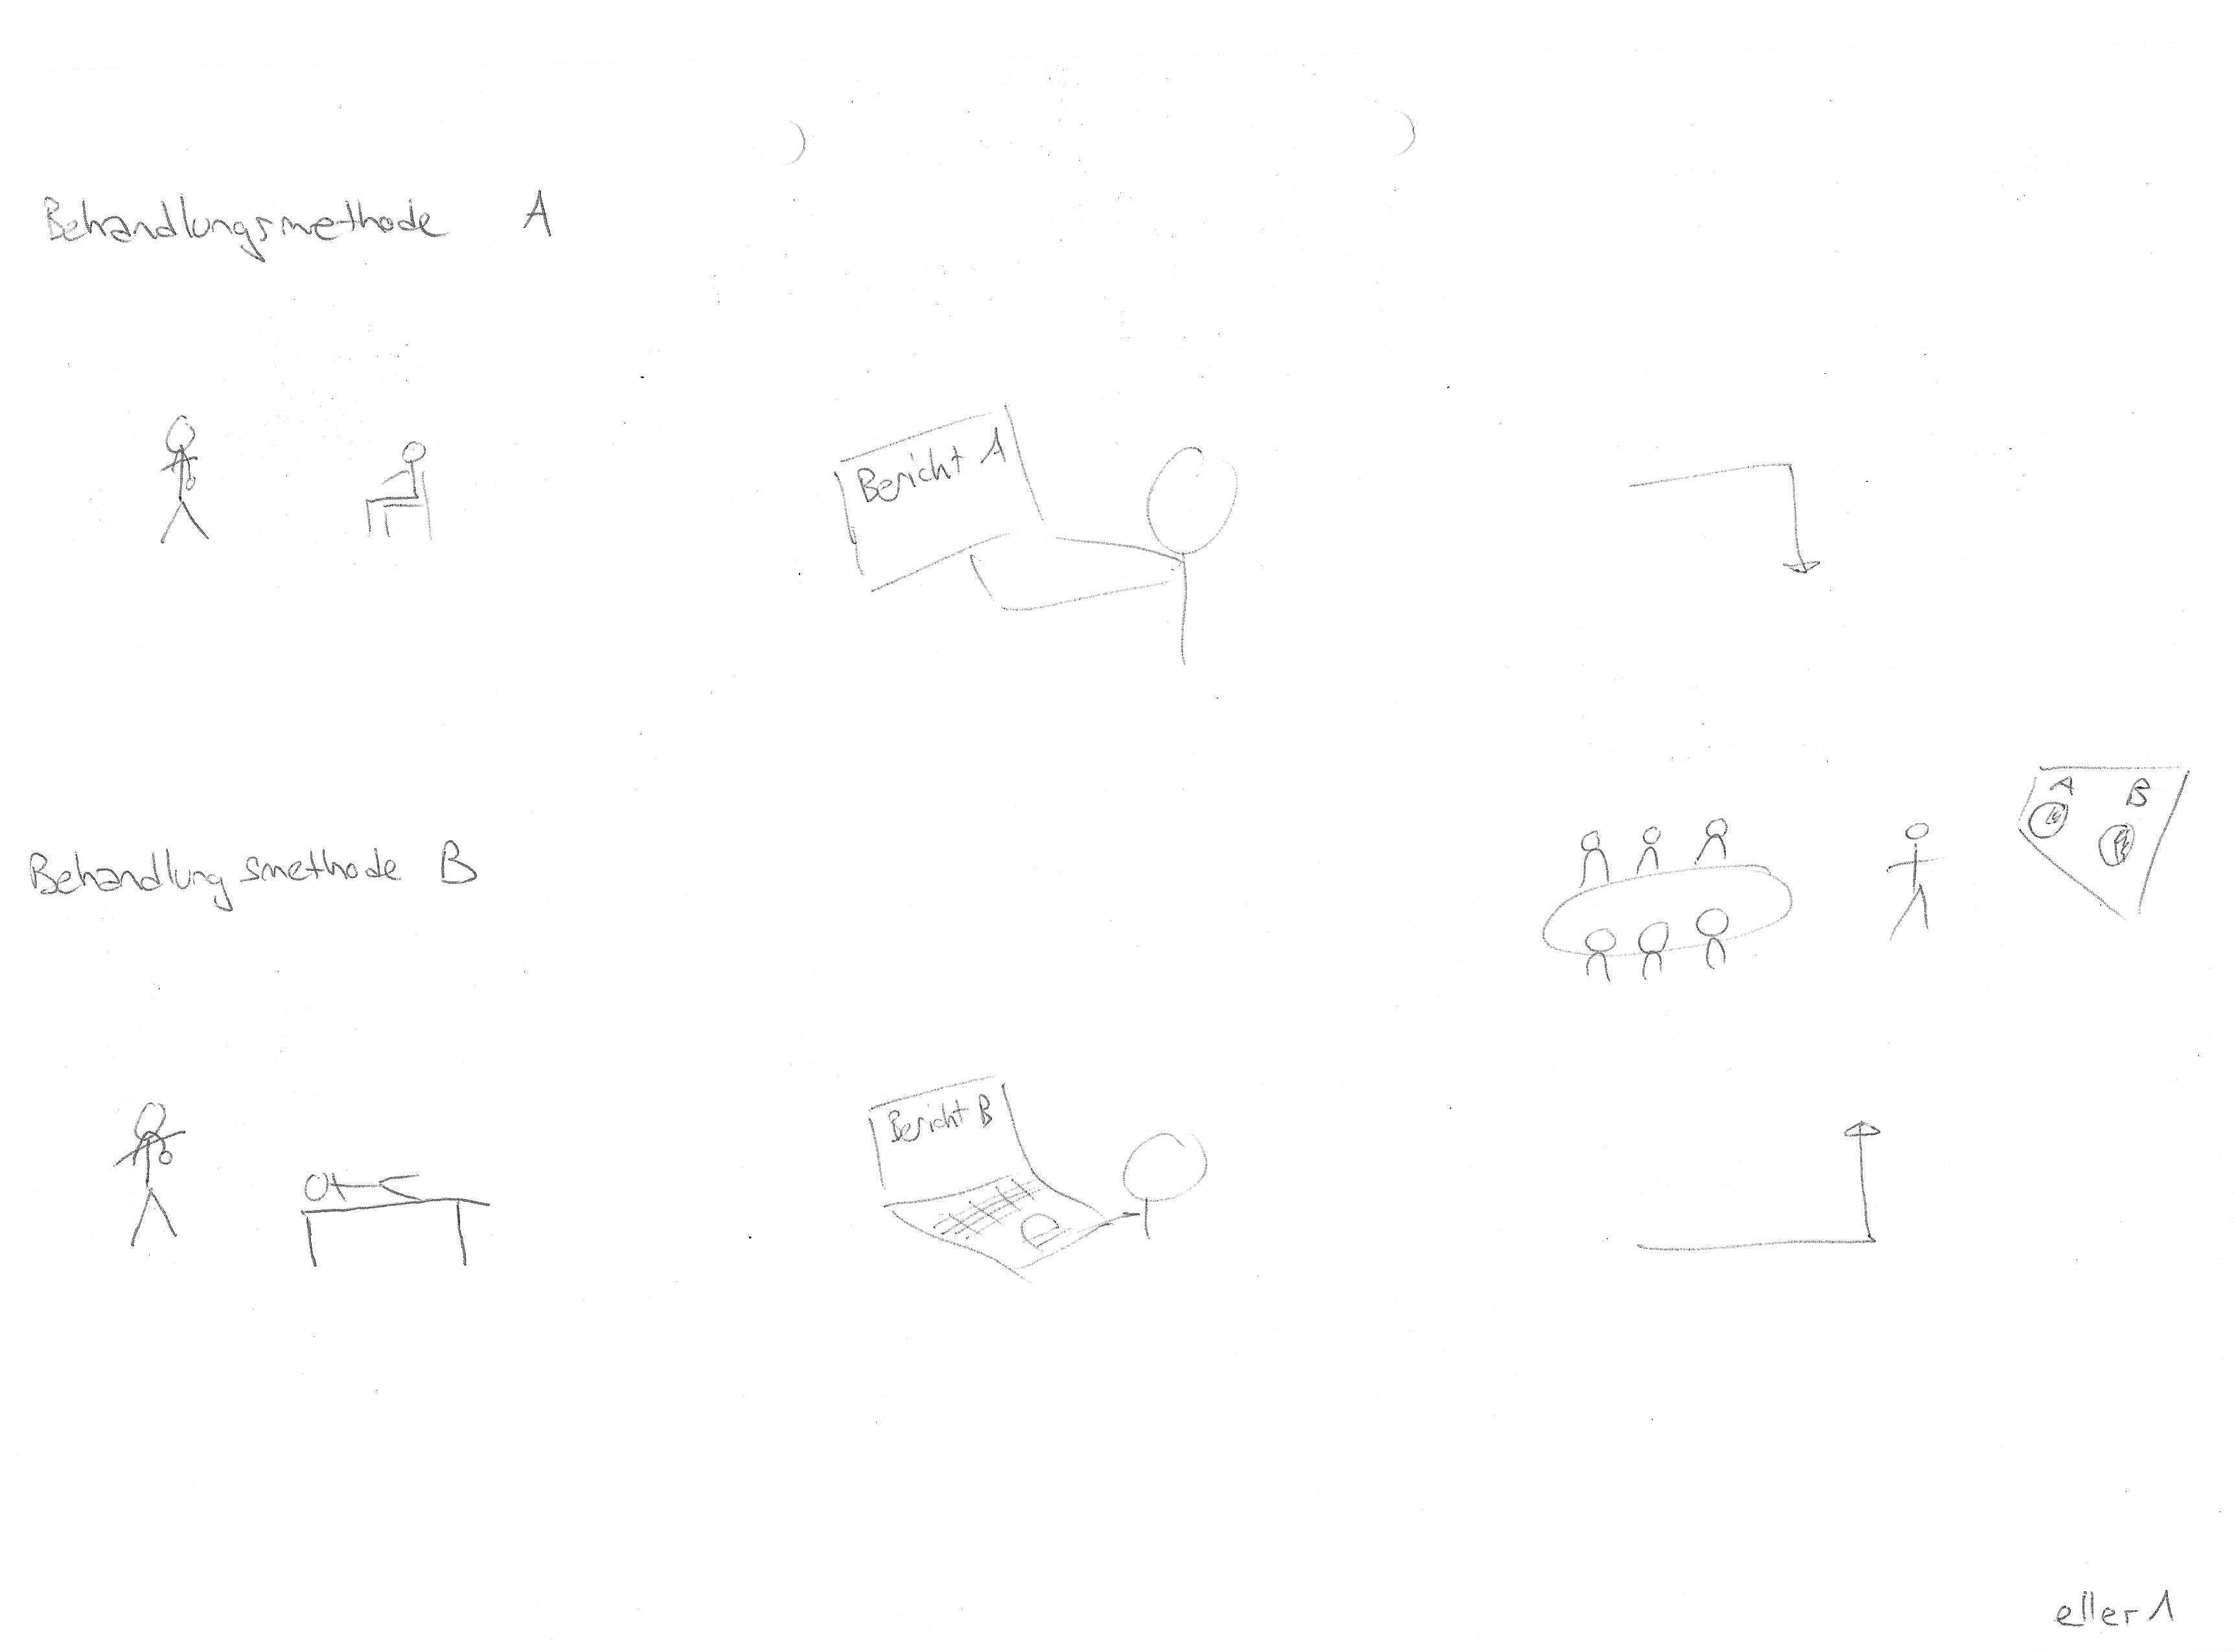
\includegraphics[width=1\textwidth]{storyboards_personas_prototypes/iteration3/eller1_storyboard2.png}

\pagebreak
\section{Prototype}
Auf Basis der oben abgebildeten Storyboards haben wir folgende Prototypen erstellt:

\paragraph{Prototyp } zu Storyboard 1\\
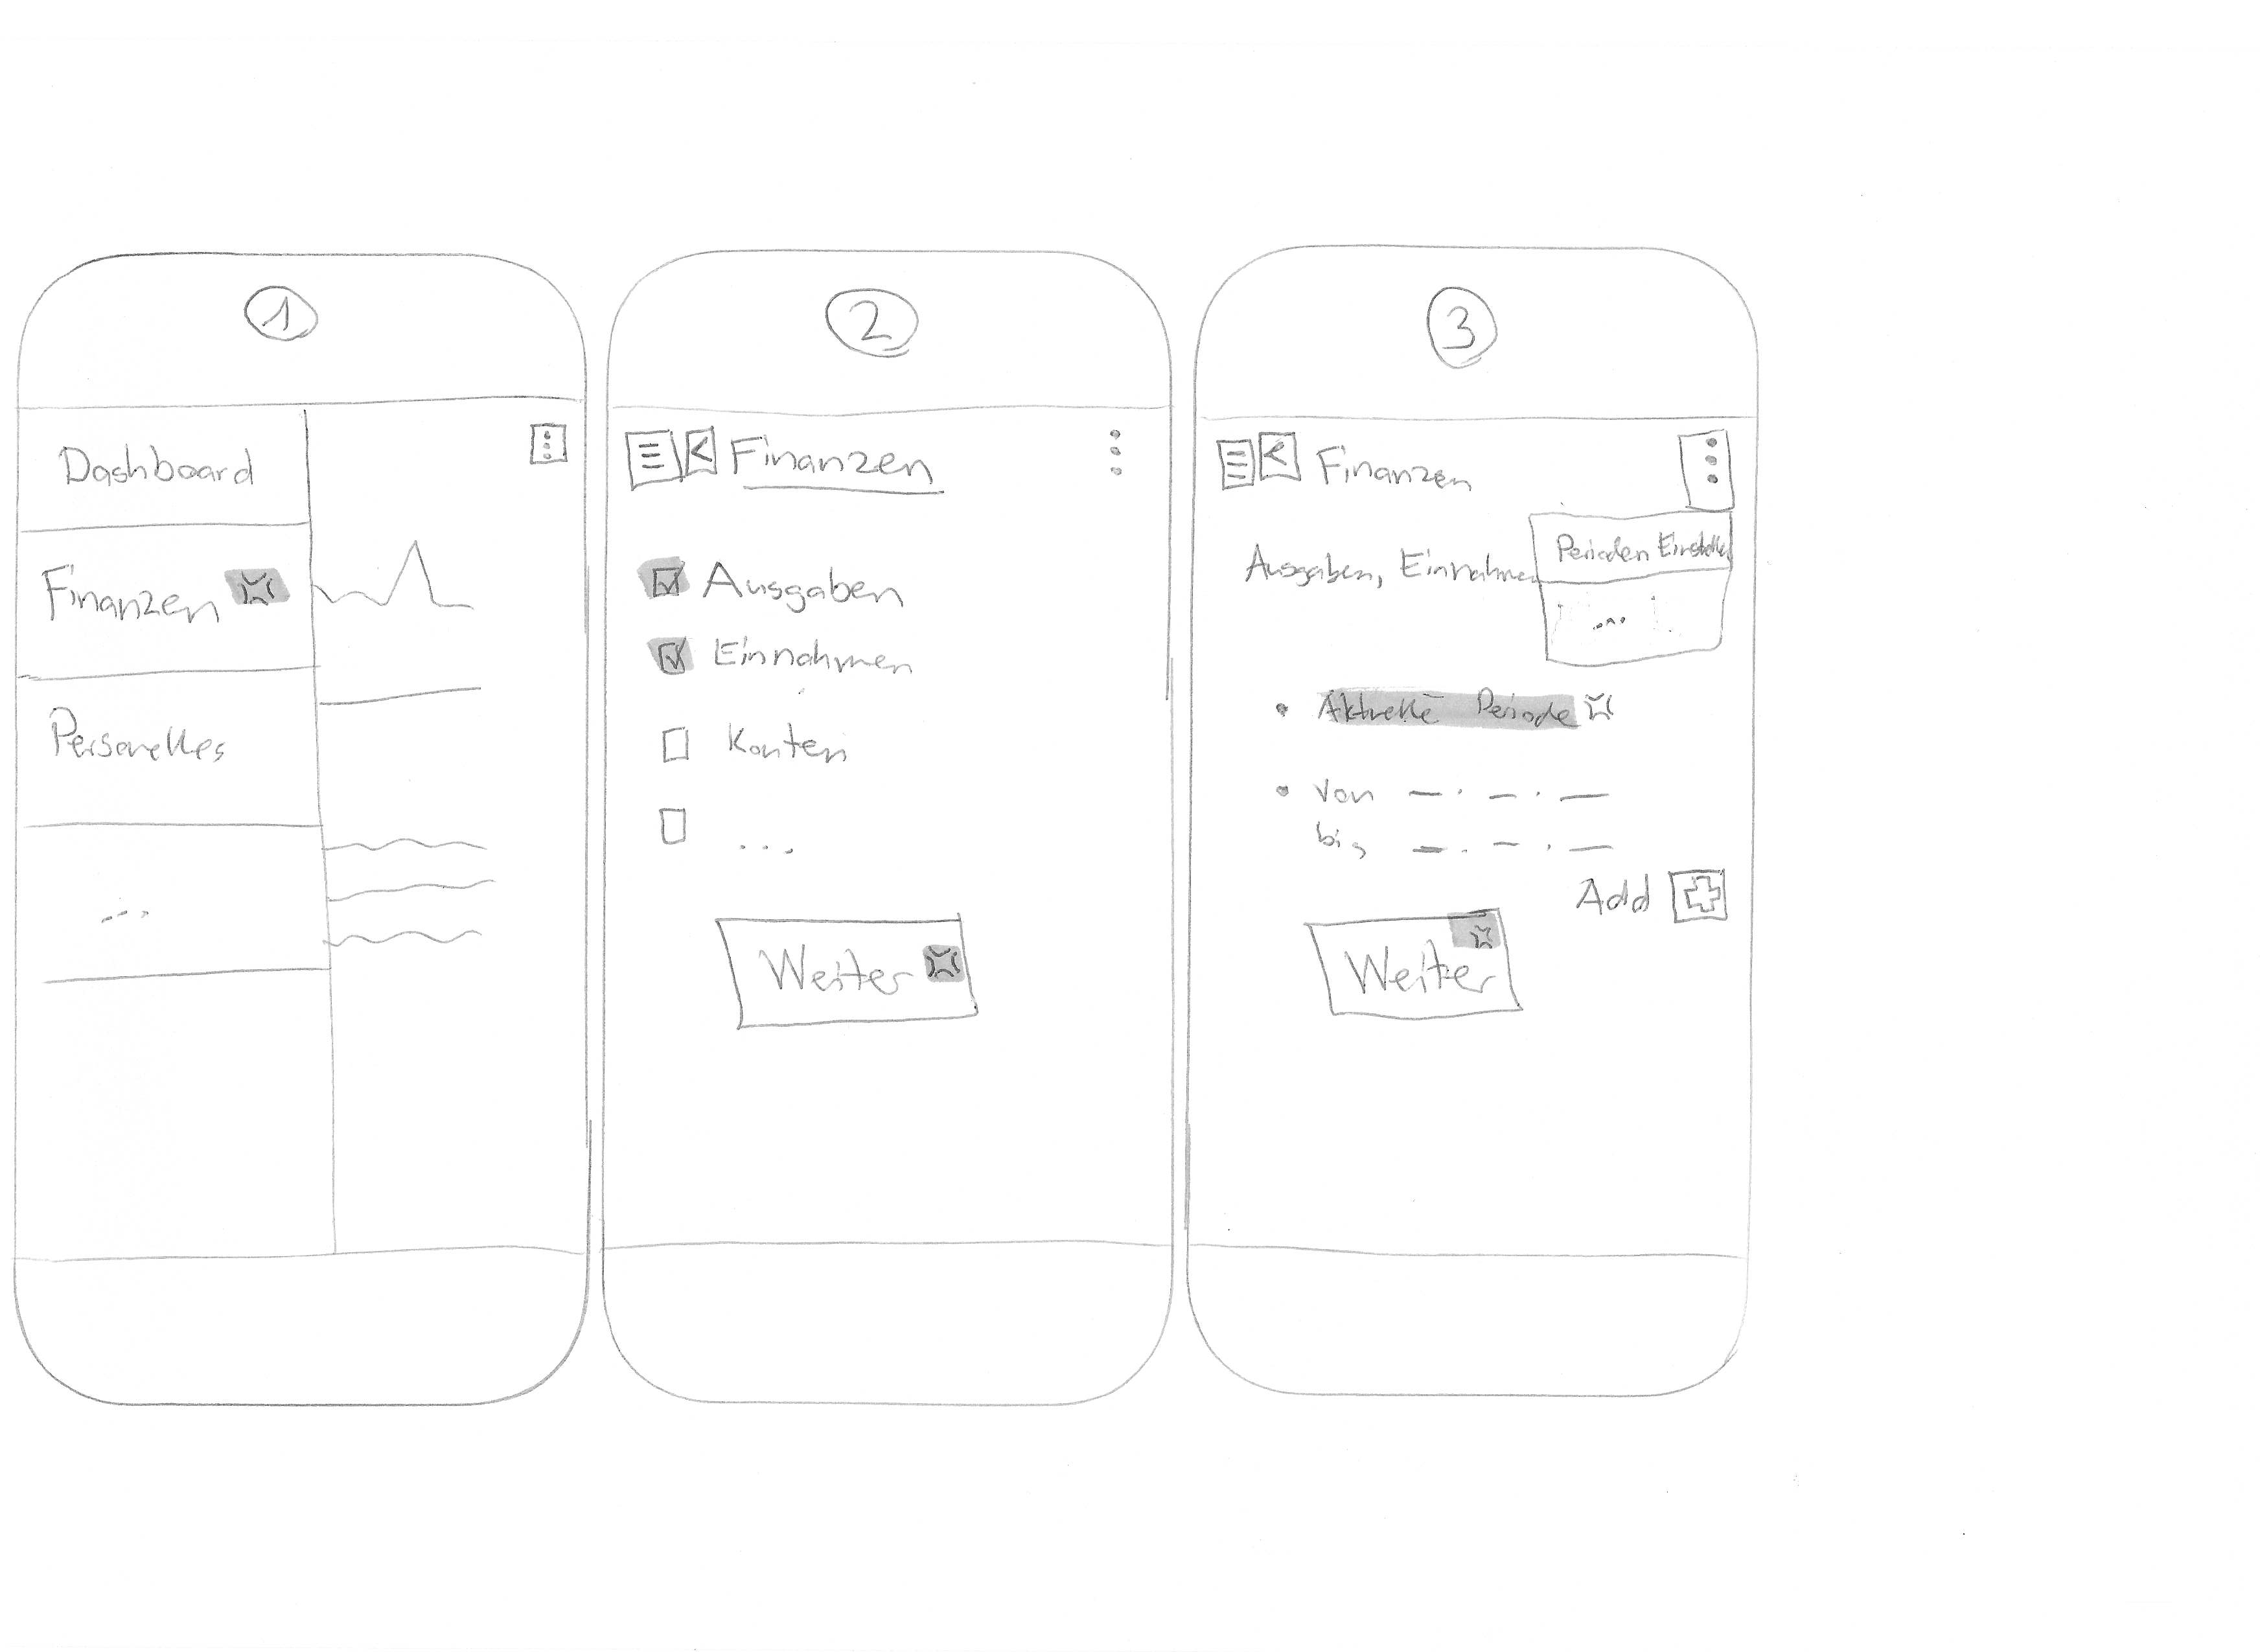
\includegraphics[width=0.85\textwidth]{storyboards_personas_prototypes/iteration3/sidlm3_storyboard2_prototype1_1.png}\\
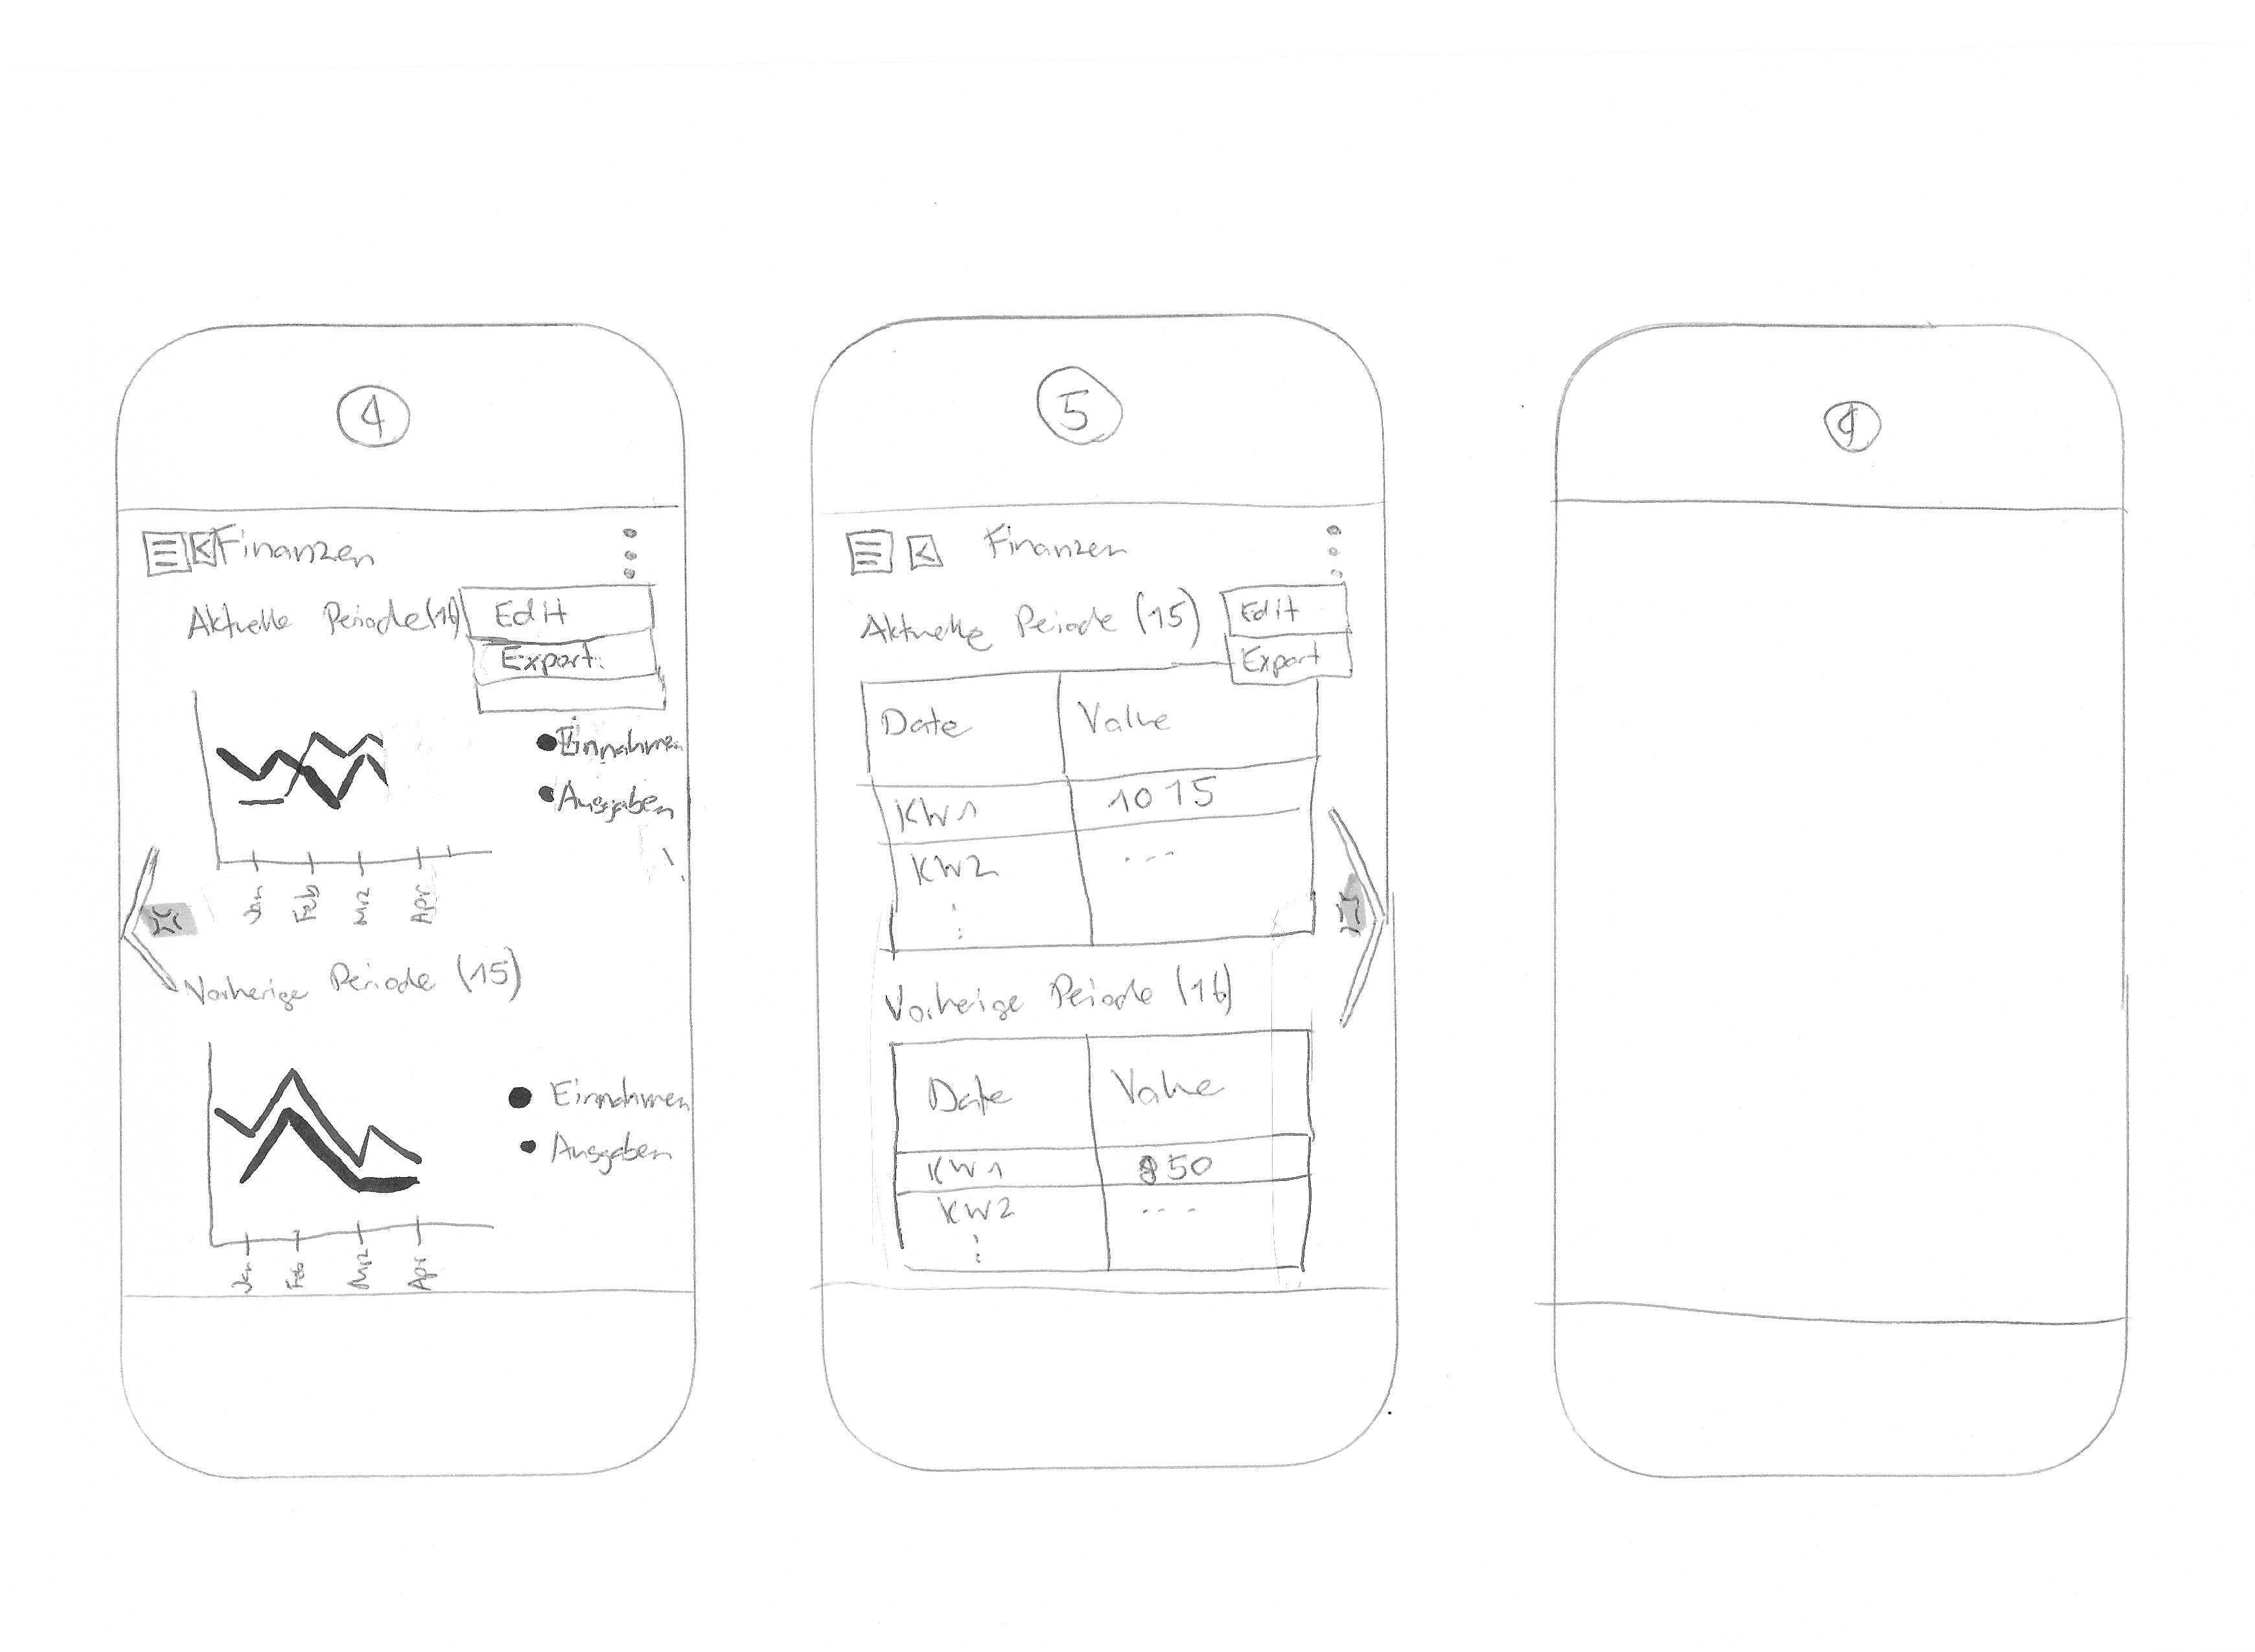
\includegraphics[width=0.85\textwidth]{storyboards_personas_prototypes/iteration3/sidlm3_storyboard2_prototype1_2.png}

\paragraph{Prototyp } zu Storyboard 2\\

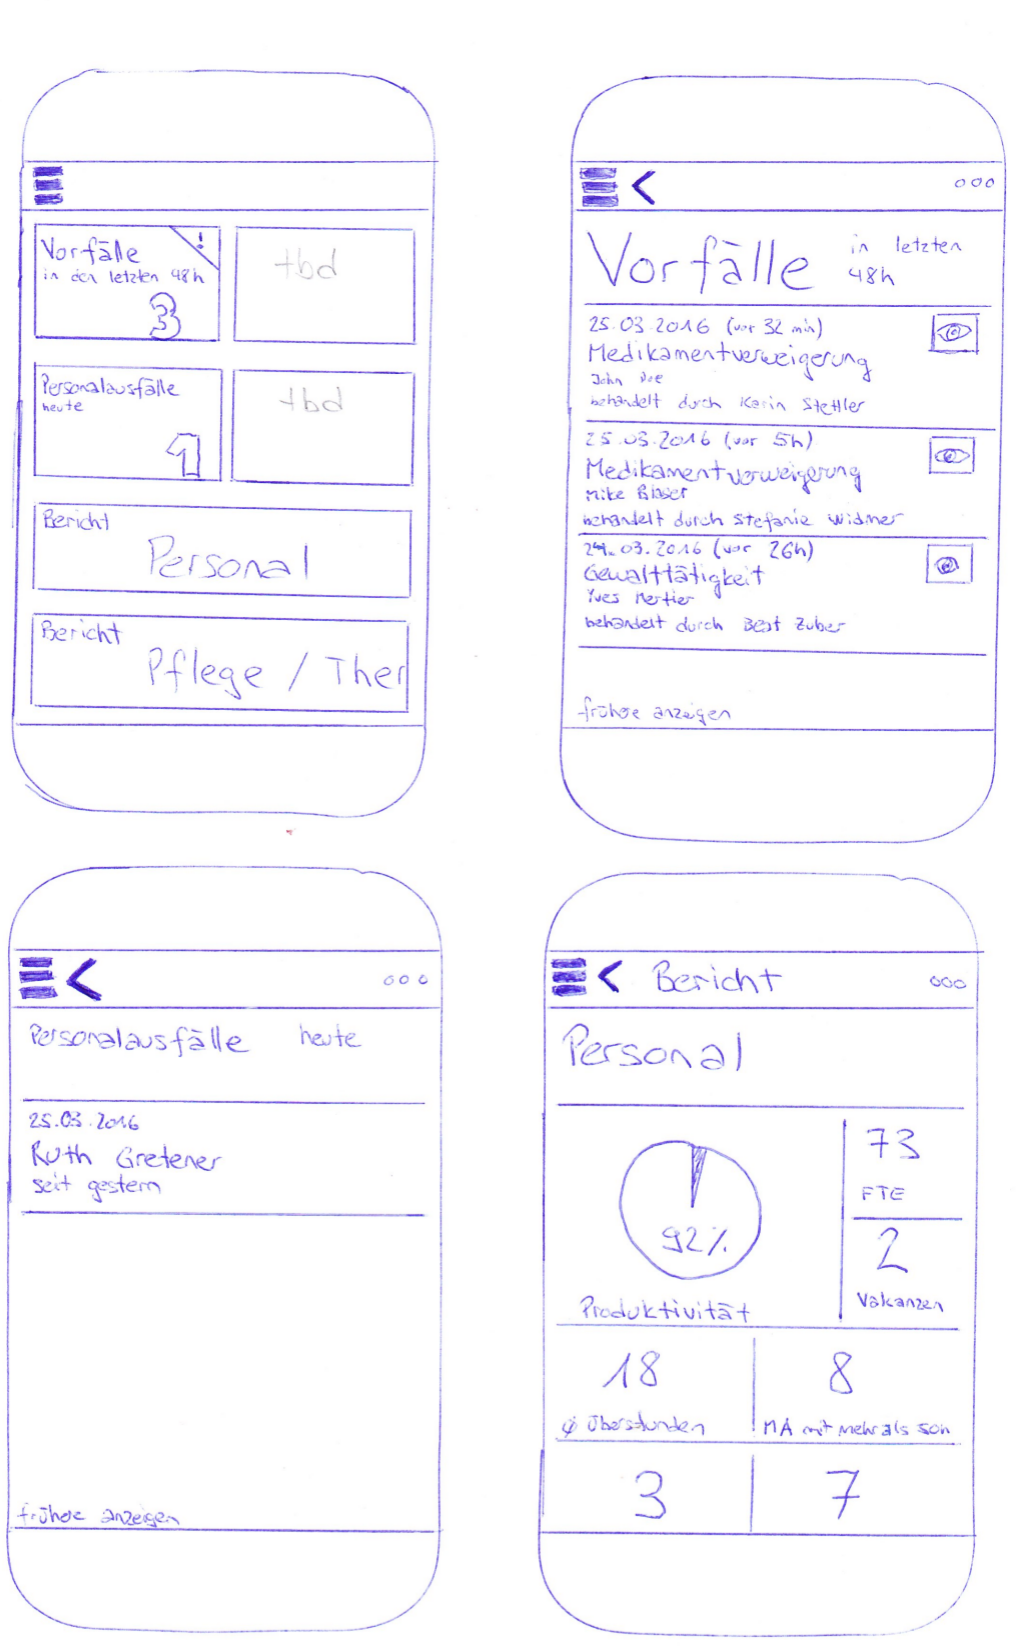
\includegraphics[width=0.48\textwidth]{storyboards_personas_prototypes/iteration3/sprim5+eller1_prototyp2_1.png}
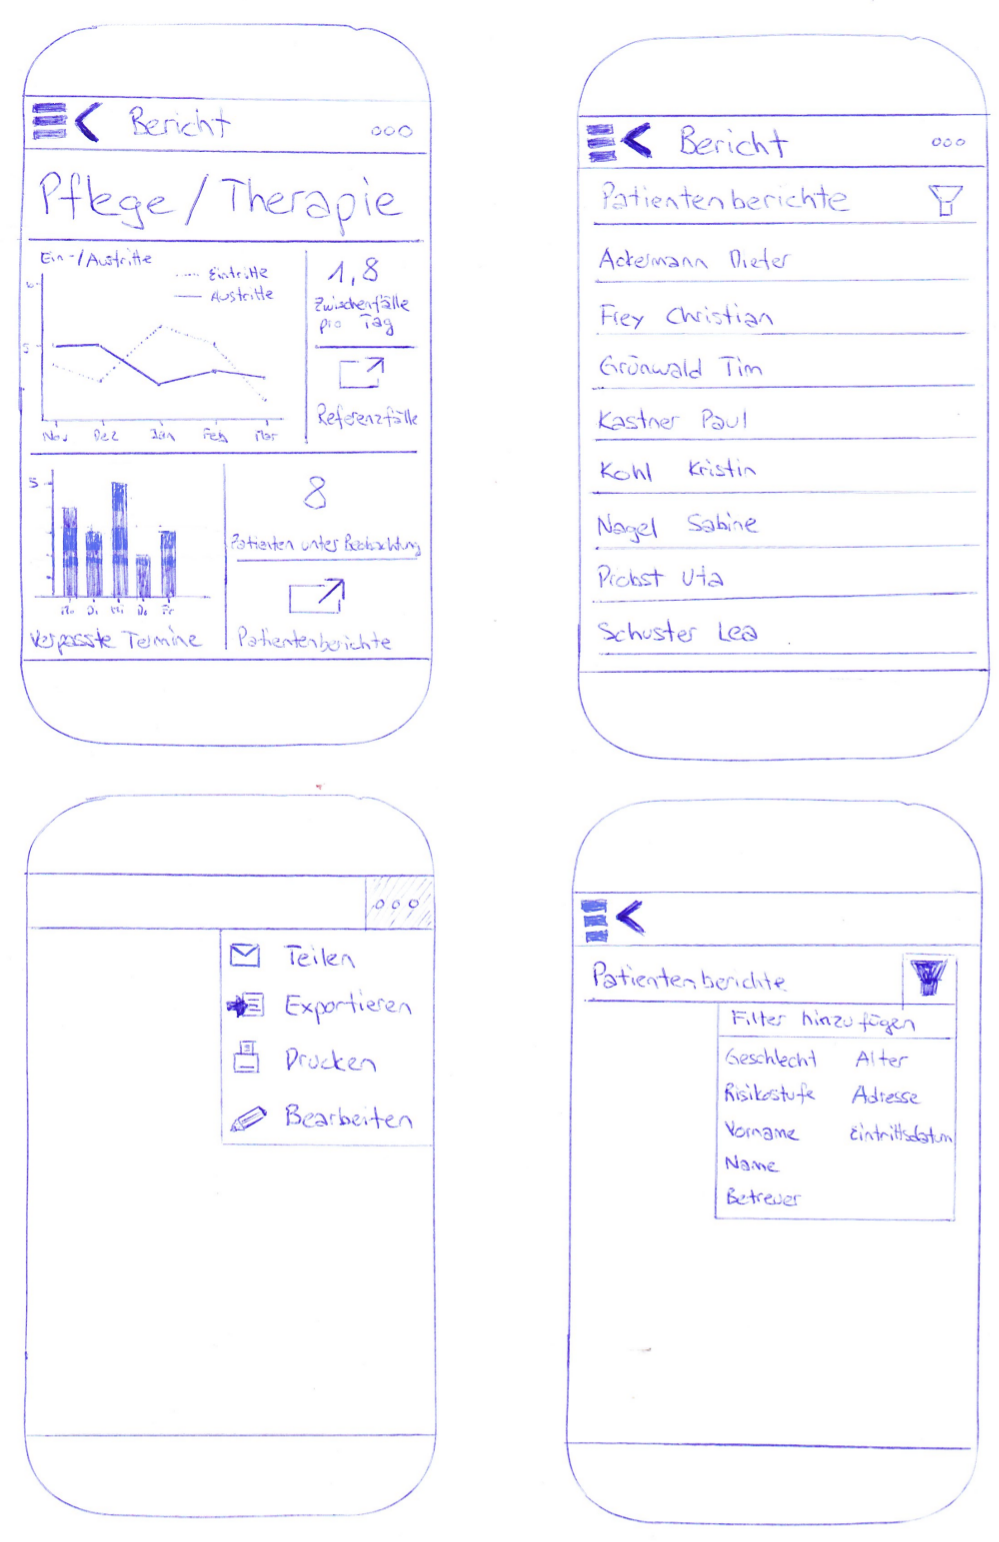
\includegraphics[width=0.48\textwidth]{storyboards_personas_prototypes/iteration3/sprim5+eller1_prototyp2_2.png}

\section{Validate}
Validierung über ein vorgefertigtes Protokoll. Die Protokolle sind im Verzeichnis der jeweilgen Iteration unter /doc/task03/storyboards\_personas\_prototypes/ abgelegt.




\end{document}